\documentclass{beamer}

%% \documentclass[handout]{beamer}
%% % use this with the [handout] option to create handouts for the audience
%% \usepackage{pgfpages}
%% \pgfpagesuselayout{2 on 1}[a4paper,border shrink=5mm]

\mode<presentation>
{
  \usetheme{Diku}
% set this to your preferences:
  \setbeamercovered{invisible}
%  \setbeamercovered{transparent}
}

\usepackage{graphicx}
\usepackage{epic}

\usepackage{amsmath}
\usepackage{amssymb}
\usepackage{amsthm}

\newcommand{\basetop}[1]{\vtop{\vskip-1ex\hbox{#1}}}
\newcommand{\source}[1]{\let\thefootnote\relax\footnotetext{\scriptsize\textcolor{kugray1}{Source: #1}}}

% for coloured code citation in text:
\usepackage{fancyvrb}

%%%%%%%%%%%%%%%%%%%%%%%%%%%%%%%%%
%%%%%    code sections   %%%%%%%%
%%%%%%%%%%%%%%%%%%%%%%%%%%%%%%%%%

% code highlighting commands in own block
\DefineVerbatimEnvironment{code}{Verbatim}{fontsize=\scriptsize}
\DefineVerbatimEnvironment{icode}{Verbatim}{fontsize=\scriptsize}

% Fancy code with color commands:
\DefineVerbatimEnvironment{colorcode}%
        {Verbatim}{fontsize=\scriptsize,commandchars=\\\{\}}

%%%%%%%%%%%%%%%%%%%%%%%%%%%%%%%%%%
%%%%%    some coloring    %%%%%%%%

\definecolor{Red}{RGB}{220,50,10}
\definecolor{Blue}{RGB}{0,51,102}
\definecolor{Yellow}{RGB}{102,51,0}
\definecolor{Orange}{RGB}{178,36,36}
\definecolor{Grey}{RGB}{180,180,180}
\definecolor{Green}{RGB}{20,120,20}
\definecolor{Purple}{RGB}{160,50,100}
\newcommand{\red}[1]{\textcolor{Red}{{#1}}}
\newcommand{\blue}[1]{\textcolor{Blue}{{#1}}}
\newcommand{\yellow}[1]{\textcolor{Yellow}{{#1}}}
\newcommand{\orange}[1]{\textcolor{Orange}{{#1}}}
\newcommand{\grey}[1]{\textcolor{Grey}{{#1}}}
\newcommand{\green}[1]{\textcolor{Green}{{#1}}}
\newcommand{\purple}[1]{\textcolor{Purple}{{#1}}}




% use "DIKU green" from our color theme for \emph
\renewcommand{\emph}[1]{\textcolor{structure}{#1}}
% use some not-too-bright red for an \emp command
\definecolor{DikuRed}{RGB}{130,50,32}
\newcommand{\emp}[1]{\textcolor{DikuRed}{ #1}}
\definecolor{CosGreen}{RGB}{10,100,70}
\newcommand{\emphh}[1]{\textcolor{CosGreen}{ #1}}
\definecolor{CosBlue}{RGB}{55,111,122}
\newcommand{\emphb}[1]{\textcolor{CosBlue}{ #1}}
\definecolor{CosRed}{RGB}{253,1,1}
\newcommand{\empr}[1]{\textcolor{CosRed}{ #1}}

\newcommand{\mymath}[1]{$ #1 $}
\newcommand{\myindx}[1]{_{#1}}
\newcommand{\myindu}[1]{^{#1}}

\newcommand{\Fasto}{\textsc{Fasto}\xspace}


%%%%%%%%%%%%%%%%%%%%

\title[Loop Parallelism]{Loop Parallelism I}

\author[C.~Oancea]{Cosmin E. Oancea\\{\tt cosmin.oancea@diku.dk}}

\institute{Department of Computer Science (DIKU)\\University of Copenhagen}

\date[Sept 2018]{September 2018 PMPH Lecture Slides}


\begin{document}

\titleslide

\input{Struct_Interm/StructLoopPar.tex}

%%%%%%%% real content starts here %%%%%%%%%%

\begin{frame}
  \frametitle{Motivation}

\begin{itemize}
    \item[+] So far we reasoned about how to parallelize a known algorithm
    \item[+] using a clean, functional approach, e.g., flattening, 
    \item[+] which provides work and depth guarantees,
    \item[\alert{-}] but does \alert{NOT} account for locality of reference.

\end  {itemize}\bigskip

\emp{Why do we have to look at imperative loops?}\pause
\begin{itemize}    
    \item A lot of legacy sequential imperative code, C{\tt++}/Java/Fortran.\medskip
    \item Need to parallelize the implementation of unknown algorithm,\medskip
    \item Need to optimize parallelism, e.g., locality of reference requires subscript analysis. 
\end  {itemize}  

\end{frame}


\section{Direction-Vector Analysis}

\begin{frame}[fragile]
	\tableofcontents[currentsection]
\end{frame}


\begin{frame}[fragile,t]
  \frametitle{Problem Statement} % of CPU, Multicores, GPGPU

%[fontsize=\small]
\begin{block}{Three Loop Examples}
\begin{colorcode}
DO i = 1, N             DO i = 2, N                 DO i = 2, N
  DO j = 1, N             DO j = 2, N                 DO j = 1, N 
    A[j,i] = A[j,i] ..      A[j,i] = A[j-1,i-1]...        A[i,j] = A[i-1,j+1]...
  ENDDO                     B[j,i] = B[j-1,i]...      ENDDO
ENDDO                   ENDDO ENDDO                 ENDDO
\end{colorcode}
\end{block} 

Iterations are ordered {\em lexicographically}, i.e., in the order
they occur in the sequential execution, e.g., 
{\tt$\vec{k}=$(i=2,j=4) < $\vec{l}=$(i=3,j=3)}.

\bigskip

\begin{itemize}
    \item \emp{Which of the three loop nests is amenable to parallelization?}\smallskip
    \item Loop interchange is one of the most simple and useful code transformations,
            e.g., used to enhance locality of reference, parallel-loop granularity,
            and even to ``create'' parallelism.\smallskip
    \item \emp{In which loop nest is it safe to interchange the loops?}
\end{itemize}


\end{frame}

\begin{frame}[fragile,t]
  \frametitle{Definition of a Dependency} % of CPU, Multicores, GPGPU
\vspace{-2ex}
\begin{block}{Load-Store Classification of Dependencies}
\begin{colorcode}
True Dependency (RAW)    Anti Dependency (WAR)    Output dependency (WAW)
S1    X  = ..            S1    .. = X             S1    X = ...            
S2    .. = X             S2    X  = ..            S2    X = ...
\end{colorcode}
\end{block} 

\smallskip

{\bf Def. Loop Dependence:} There is a dependence from statement $S1$ to $S2$
in a loop nest {\em iff} $\exists$ iterations $\vec{k}$, $\vec{l}$ such that:\pause
\begin{description}
    \item[1.] $\vec{k} < \vec{l}$ or $\vec{k} = \vec{l}$ and $\exists$ 
                an execution path from statement $S1$ to statement $S2$ \emp{such that:}
    \item[2.] $S1$ accesses memory location $M$ on iteration $\vec{k}$, and
    \item[3.] $S2$ accesses memory location $M$ on iteration $\vec{l}$, and
    \item[4.] one of these accesses is a write.
\end{description}
\medskip

\emp{We say that $S1$ is the source and $S2$ is the sink of the dependence}, 
because $S1$ executes before $S2$ in the sequential program execution.
Dependence depicted with an arrow pointing from source to sink.\pause

\medskip
We are most interested in cross iteration dependencies, i.e., $\vec{k} < \vec{l}$.\\\smallskip
Intra iteration dependencies, i.e., $\vec{k} = \vec{l}$ are analysed for ILP. 

\end{frame}


\begin{frame}[fragile,t]
  \frametitle{Loop-Nest Dependencies} % of CPU, Multicores, GPGPU

{\em Lexicographic ordering}, 
e.g., {\tt$\vec{k}=$(i=2,j=4) < $\vec{l}=$(i=3,j=3)}.

%[fontsize=\small]
\begin{block}{Three Loop Examples}
\begin{colorcode}
DO i = 1, N             DO i = 2, N                 DO i = 2, N
  DO j = 1, N             DO j = 2, N                 DO j = 1, N 
    A[j,i] = A[j,i] ..      A[j,i] = A[j-1,i-1]...        A[i,j] = A[i-1,j+1]...
  ENDDO                     B[j,i] = B[j-1,i]...      ENDDO
ENDDO                   ENDDO ENDDO                 ENDDO
\end{colorcode}
\end{block} 
\pause

\hspace{-3ex}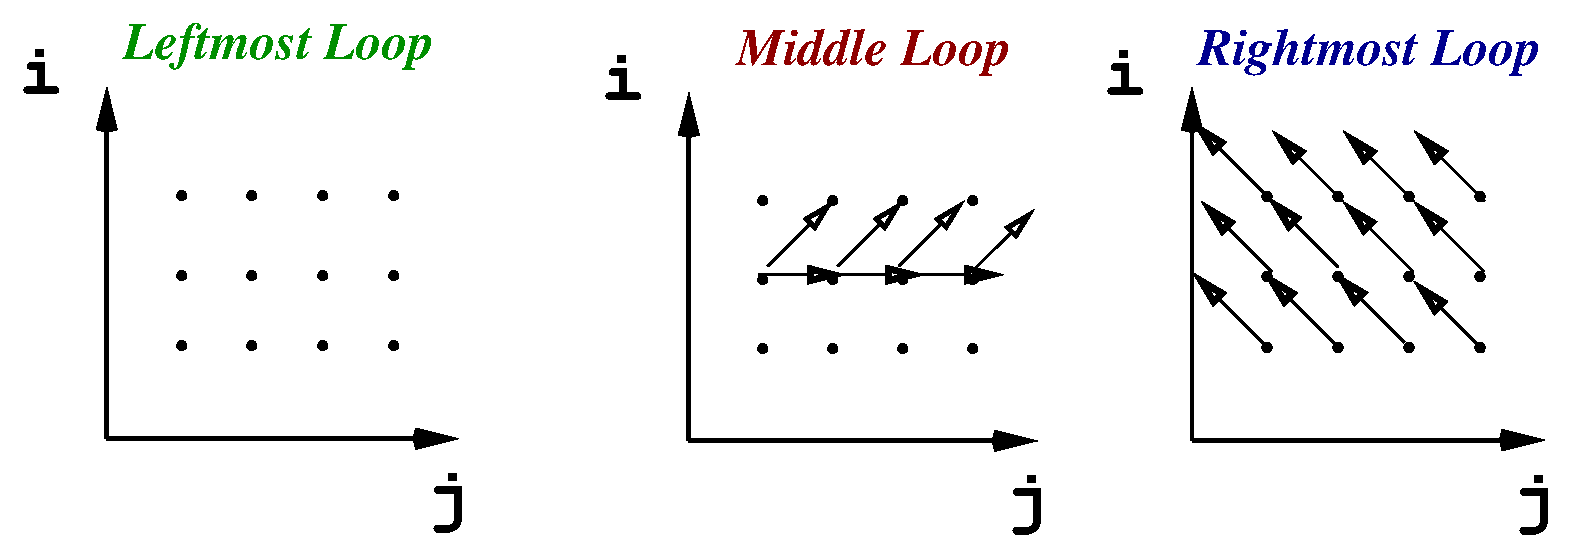
\includegraphics[height=23ex]{Figures/L5-LoopPar/LoopDeps}  

\alert{How can I summarize this information?} %Do I have to consider all cases?

\end{frame}





\begin{frame}[fragile,t]
  \frametitle{Aggregate Dependencies via Direction Vectors} % of CPU, Multicores, GPGPU

\begin{block}{Write the Direction Vectors for Each Loop:}
\begin{colorcode}
  DO i = 1, N            DO i = 2, N               DO i = 2, N
    DO j = 1, N            DO j = 2, N               DO j = 1, N 
S1    A[j,i]=A[j,i]..  S1   A[j,i]=A[j-1,i]...   S1    A[i,j]=A[i-1,j+1]...
    ENDDO              S2   B[j,i]=B[j-1,i-1]...     ENDDO
  ENDDO                  ENDDO ENDDO               ENDDO
\end{colorcode}
\end{block} 



\smallskip

Dependencies depicted via an edge {\em from} the stmt that executes first
in the loop nest, i.e., {\em the source}, {\em to} the one that executes later, {\em the sink}.

\smallskip

{\bf Def. Dependence Direction:} Assume $\exists$ a dependence from $S1$ in iteration $\vec{k}$
to $S2$ in $\vec{l}$ ($\vec{k}\leq\vec{l}$). 
\emp{\em Dependence-direction vector $\vec{D}(\vec{k},\vec{l})$}:
\begin{description}
    \item[1.] $\vec{D}(\vec{k},\vec{l})_m = $~``{\tt{}<}'' if $\vec{k}_m < \vec{l}_m$,
    \item[2.] $\vec{D}(\vec{k},\vec{l})_m = $~``{\tt{}=}'' if $\vec{k}_m = \vec{l}_m$,
    \item[3.] $\vec{D}(\vec{k},\vec{l})_m = $~``{\tt{}>}'' if $\vec{k}_m > \vec{l}_m$.
\end{description}

\medskip
If the source is a write and the sink a read then {\sc raw} dependency,\\iIf the source is a read then {\sc war}, if both are writes then {\sc waw}.  
\end{frame}


\begin{frame}[fragile,t]
  \frametitle{How to Compute the Direction Vectors?}
\begin{itemize}
    \item For any two statements $S1$ and $S2$ that may access the same
            array $A$ (and one of the accesses is a write),\medskip
    \item in two symbolic iterations $I^1\equiv(i^1_1,\ldots i^1_m)$
            and $I^2=(i^2_1,\ldots i^2_m)$ (such that $I^1 < I^2$)\medskip
    \item on indices $A[e^1_1,\ldots,e^1_n]$ and $A[e^2_1,\ldots,e^2_n]$,
            respectivelly,\medskip
    \item then \textbf{\it the direction vectors may be derived} from the equations\\
            $\begin{cases}
                e^1_1 = e^2_1\\
                \ldots\\
                e^1_n = e^2_n
            \end{cases}$\\
            (The system of equations models the definition of a dependency: 
                both accesses need to refer to the same memory location!)
\end{itemize}
\end{frame}

\begin{frame}[fragile,t]
  \frametitle{Parallelism and Loop Interchange} % of CPU, Multicores, GPGPU

\begin{block}{Direction Vectors/Matrix for Three Loops }
\begin{columns}
\column{0.27\textwidth}
\begin{colorcode}
  DO i = 1, N
    DO j = 1, N
S1    A[j,i]=A[j,i]..
    ENDDO
  ENDDO\pause
For S1\mymath{\rightarrow}S1: 
    (j1,i1)=(j2,i2) 
    i1 \emp{=} i2 \& j1 \emp{=} j2

Direction matrix:
S1\mymath{\rightarrow}S1: \emp{[=,=]}
\end{colorcode}
\column{0.32\textwidth}
\begin{colorcode}
  DO i = 2, N
    DO j = 2, N
S1    A[j,i]=A[j-1,i]...
S2    B[j,i]=B[j-1,i-1]...
    ENDDO
  ENDDO\pause
S1\mymath{\rightarrow}S1: (j1,i1)=(j2-1,i2)
        i1 \emp{=} i2 \& j1 \emp{<} j2
S2\mymath{\rightarrow}S2: (j1,i1)=(j2-1,i2-1)
        i1 \emp{<} i2 \& j1 \emp{<} j2
S1\mymath{\rightarrow}S1: \emp{[=,<]}
S2\mymath{\rightarrow}S2: \emp{[<,<]}
\end{colorcode}
\column{0.32\textwidth}
\begin{colorcode}
  DO i = 2, N
    DO j = 1, N
S1    A[i,j]=A[i-1,j+1]...
    ENDDO
  ENDDO
For S1\mymath{\rightarrow}S1:\pause
    (i1,j1) = (i2-1,j2+1)
    i1 \emp{<} i2 \& j1 \emp{>} j2

Direction matrix:
S1\mymath{\rightarrow}S1: \emp{[<,>]}
\end{colorcode}
\end{columns}
\end{block} 

{\bf Th. Parallelism:} A loop in a loop nest is parallel {\em iff} all its directions
are either {\tt =} or there exists an outer loop whose corresp. direction is {\tt <}. 

\smallskip

\alert{A direction vector cannot have $>$ as the first non-= symbol},\\
as that would mean that I depend on something in the future. 
\end{frame}

\begin{frame}[fragile,t]
  \frametitle{Parallelism and Loop Interchange} % of CPU, Multicores, GPGPU

\begin{block}{Direction Vectors/Matrix for Three Loops }
\begin{columns}
\column{0.27\textwidth}
\begin{colorcode}
  DO i = 1, N
    DO j = 1, N
S1    A[j,i]=A[j,i]..
    ENDDO
  ENDDO
For S1\mymath{\rightarrow}S1: 
    (j1,i1)=(j2,i2) 
    i1 \emp{=} i2 \& j1 \emp{=} j2

Direction matrix:
S1\mymath{\rightarrow}S1: \emp{[=,=]}
\end{colorcode}
\column{0.32\textwidth}
\begin{colorcode}
  DO i = 2, N
    DO j = 2, N
S1    A[j,i]=A[j-1,i]...
S2    B[j,i]=B[j-1,i-1]...
    ENDDO
  ENDDO
S1\mymath{\rightarrow}S1: (j1,i1)=(j2-1,i2)
        i1 \emp{=} i2 \& j1 \emp{<} j2
S2\mymath{\rightarrow}S2: (j1,i1)=(j2-1,i2-1)
        i1 \emp{<} i2 \& j1 \emp{<} j2
S1\mymath{\rightarrow}S1: \emp{[=,<]}
S2\mymath{\rightarrow}S2: \emp{[<,<]}
\end{colorcode}
\column{0.32\textwidth}
\begin{colorcode}
  DO i = 2, N
    DO j = 1, N
S1    A[i,j]=A[i-1,j+1]...
    ENDDO
  ENDDO
For S1\mymath{\rightarrow}S1: 
    (i1,j1) = (i1-1,j2+1)
    i1 \emp{<} i2 \& j1 \emp{>} j2

Direction matrix:
S1\mymath{\rightarrow}S1: \emp{[<,>]}
\end{colorcode}
\end{columns}
\end{block} 

{\bf Th. Loop Interchange:} A column permutation of the loops in a loop nest 
is legal {\em iff} permuting the direction matrix in the same way {\em does NOT result}
in a {\tt >} direction as the leftmost non-{\tt{}=} direction in a row. 

\end{frame}


\begin{frame}[fragile,t]
  \frametitle{Parallelism and Loop Interchange} 

\begin{block}{Direction Vectors/Matrix for Three Loops }
\begin{colorcode}
  DO i = 1, N            DO i = 2, N               DO i = 2, N
    DO j = 1, N            DO j = 2, N               DO j = 1, N 
S1    A[j,i]=A[j,i]..  S1   A[j,i]=A[j-1,i]...   S1    A[i,j]=A[i-1,j+1]...
    ENDDO              S2   B[j,i]=B[j-1,i-1]...     ENDDO
  ENDDO                  ENDDO ENDDO               ENDDO

For S1\mymath{\rightarrow}S1: j1 = j2    For S1\mymath{\rightarrow}S1: j1 = j2-1          For S1\mymath{\rightarrow}S1: i1 = i2-1
            i1 = i2                i1 = i2                    j1 = j2+1
(i2,j2)-(i1,j1)=         (i2,j2)-(i1,j1)=\emp{[=,<]}        (i2,j2)-(i1,j1)=\emp{[<,>]}
\emp{[=,=]}                  For S2\mymath{\rightarrow}S2: j1 = j2-1
                                   i1 = i2-1
                         (i2,j2)-(i1,j1)=\emp{[<,<]}
\end{colorcode}
\end{block} 

Interchange is safe for the first and second nests, but not for the third!\\
e.g., \emp{\tt [=,<]}$~~~\rightarrow~~~$ \emph{\tt [<,=]}$~~~~~~~~~$(for the second loop nest)\\
$~~~~~~$\emp{\tt [<,<]}$~~~~~~~~~~~~$\emph{\tt [<,<]}

\pause\smallskip

After interchange, loop $j$ of the second loop nest is parallel.

\bigskip

\emph{\bf Corollary: A parallel loop can be always interchanged inwards.}
\end{frame}


\begin{frame}[fragile,t]
  \frametitle{Dependency Graph and Loop Distribution} 

{\bf Def. Dependency Graph:} edges from the source of the dependency, i.e., early iteration, 
to the sink, i.e., later iteration. 

\smallskip

{\bf Th. Loop Distribution:} Statements that are in a dependence cycle remain in one 
(sequential) loop.   The others are distributed to separate loops in graph order; 
if no cycle then parallel loops.\smallskip

\begin{block}{Vectorization Example: Remember Vector Machines?}
\begin{columns}
\column{0.34\textwidth}
\begin{colorcode}[fontsize=\scriptsize]
  DO i = 3, N
\emp{S1  A[i] = B[i-2] ...}
\alert{S2  B[i] = B[i-1] ...}
  ENDDO  

For S2\mymath{\rightarrow}S1: i1 = i2-2, \emp{[<]}
For S2\mymath{\rightarrow}S2: i1 = i2-1, \emp{[<]}
\end{colorcode}
\column{0.27\textwidth}\pause
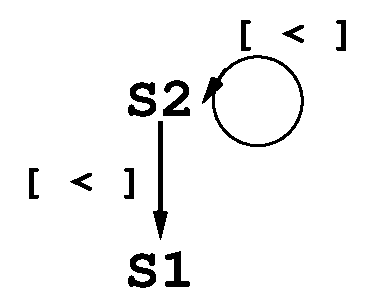
\includegraphics[height=12ex]{Figures/L5-LoopPar/LoopDistr}  
\column{0.30\textwidth}
\begin{colorcode}[fontsize=\scriptsize]
  \alert{DO} i = 3, N
S2  B[i] = B[i-1] ...
  \alert{ENDDO}

  \emphh{DOALL} i = 3, N
\emp{S1  A[i] = B[i-2] ...}
  \emphh{ENDDOALL}
\end{colorcode}
\end{columns}
\end{block}

\medskip

{\bf Corollary:} It is always legal to distribute a parallel loop;\\
\alert{but requires array expansion for local variables or if output
dependencies are present.}
\end{frame}

\begin{frame}[fragile,t]
  \frametitle{Loop Distribution May Require Array Expansion} 


\begin{columns}
\column{0.4\textwidth}
\begin{colorcode}[fontsize=\scriptsize]
  float tmp;
  for(i=2; i<N; i++) \{
    \emp{tmp} = 2*B[i-2]; 
    A[i] = tmp;
    B[i] = tmp+B[i-1]
  \}
\end{colorcode}
\column{0.53\textwidth}
\begin{colorcode}[fontsize=\scriptsize]
  \emph{float tmp[N]};
  for(int i=2; i<N; i++) \{
    tmp[i] = 2*B[i-2]; 
    B[i] = tmp[i]+B[i-1];
  \}

  \emph{forall(int i=2; i<N; i++)} \{
    A[i] = tmp[i];
  \}
\end{colorcode}
\end{columns}
\bigskip

No matter where {\tt tmp} is declared (inside or outside
the loop) it needs to be expanded into an array in order
to do loop distribution.\bigskip

If {\tt tmp} is declared outside the loop then requires \emp{\bf privatization}, \pause
because it actually causes frequent {\sc waw} dependencies.
However its value is written before being used within the same iteration.
Hence it is semantically equivalent to a locally declared variable,
which will remove the output ({\sc waw}) dependency.\bigskip

Distribution requires array expansion of the scalar {\tt tmp}.

\end{frame}


\begin{frame}[fragile,t]
  \frametitle{False Dependencies (WAR/WAW)} 

\begin{itemize}
    \item \emp{Cross-Iteration Anti Dependencies (WAR)} 
        correspond to a read from the array as it was 
        before the loop $\Rightarrow$ can be eliminated
        by reading from a copy of the array.\bigskip

    \item \emp{Cross-Iteration WAW Dependencies (WAW)}:\\
        If they correspond to the case in which every \emp{\bf read} from
        a scalar or array location is covered by a \emp{\bf previous same-iteration write}
        %a re-writing the same array elements
        %in different iterations 
        $\Rightarrow$ can be eliminated \emph{\bf privatization (renaming)},
        which semantically moves the declaration of the variable (scalar or array) 
        inside the loop.\bigskip

    \item Direction-vectors reasoning is limited to relatively
        simple loop nests, e.g., difficult to reason about 
        privatization in such a way.
\end  {itemize}
\end{frame}

\begin{frame}[fragile,t]
  \frametitle{Example: Eliminating WAR Dependencies} 

\begin{block}{Anti Dependency (WAR) {\tt~~} and {\tt~~}Output Dependency (WAW)}
\begin{columns}
\column{0.40\textwidth}
\begin{colorcode}[fontsize=\scriptsize]
  float tmp = A[1];
  \emp{for (i=0; i<N-1; i++)}
\emp{S1  A[i] = A[i+1];} 
  A[N-1] = tmp;

//S1\mymath{\rightarrow}S1: i1+1=i2, \emp{[<]} WAR\pause
\end{colorcode}

\column{0.55\textwidth}
\begin{colorcode}[fontsize=\scriptsize]
// Solution: copy A into A'
// and use A' for the reads!
float Acopy[N];
\#pragma omp parallel for
  \emph{for(i=0; i<N; i++)} \{
    Acopy[i] = A[i];
  \}
  tmp = A[1];
\emph{\#pragma omp parallel for} \emp{private(i)}
  for (i=0; i<N-1; i++) \{
    \emph{A[i] = Acopy[i+1];}
  \}
  A[N-1] = tmp;
\end{colorcode}
\end{columns}
\end{block}

%free(A);

For OpenMP code, run the g++ compiler with the {\tt -fopenmp} flag.\\
You may play with the degree of parallelism by setting the {\tt OMP\_NUM\_THREADS}
enviornment variable, e.g., to run on $4$ cores use:\\
{\tt \$ export OMP\_NUM\_THREADS=4}.

\end{frame}



\begin{frame}[fragile,t]
  \frametitle{Example: Eliminating WAW Dependencies} 

\begin{block}{Anti Dependency (WAR) {\tt~~} and {\tt~~}Output Dependency (WAW)}
\begin{columns}
\column{0.40\textwidth}
\begin{colorcode}[fontsize=\scriptsize]
  int A[M];
  for(i=0; i<N; i++)\{
    for(int j=0, j<M; j++)
        \emp{A[j]} = (4*i+4*j) \% M;
    for(int k=0; k<N; k++)
        X[i,k] = X[i,k-1] * 
                 \emp{A[A[(2*i+k)\%M]\%M]};
  \}\pause
\end{colorcode}

\column{0.55\textwidth}
\begin{colorcode}[fontsize=\scriptsize]
// \emp{The write to A[j] causes multiple WAWs},\pause
// \emph{but A is fully written in the inner loop} 
\emph{\#pragma omp parallel}\{
  int A[M];
\emph{\#pragma omp for}
  for(int i=0; i<N; i++)\{
    for(int j=0, j<M; j++)
        \emp{A[j]} = (4*i+4*j) \% M;
    for(int k=0; k<N; k++)
        X[i,k]=X[i,k-1] * 
               \emp{A[A[(2*i+k)\%M]\%M]};
  \}
\}
\end{colorcode}
\end{columns}
\end{block}

The declaration of {\tt in A[M]} inside the OMP parallel region,
will create an array {\tt A} for every thread (and visible/accessible
inside the thread context).\smallskip

Alternatively you may expand {\tt A} with a new dimension of
number-of-processor size, and use explicit indexing.
  %free(A);

\end{frame}

\begin{frame}[fragile,t]
  \frametitle{Reduction is Typically Easy To Recognize} 

If all the statements in which a scalar variable {x} appears
are of the form {\tt x $\oplus$ = $exp$}, where {\tt x} does 
not appear in $\exp$ and $\oplus$ is associative 
then the cross-iteration RAWs on {\tt x} can be resolved by:
\begin{itemize}
    \item privatizing {\tt x} initialized with the neutral element,
    \item computing the per-processor partial values of {\tt x},
    \item reducing the {\tt x}s across processors and with the initial value.
\end  {itemize} 

\begin{columns}
\column{0.4\textwidth}
\begin{colorcode}[fontsize=\scriptsize]
// compilation requires g++ -fopenmp ...
  float x = 6.0;
\#pragma omp parallel for reduction(+:x) private(i,j)
  for(i=1; i<N; i++) \{
    for(j=1; j<N; j++) \{
      if ( A[i,j] >= 2.0 )    \emph{x += 2*A[i,j-1]};
      else if( A[i,j] > 0.0 ) \emph{x += A[i-1,j+1];}
    \}
    if (i \% (j+1) == 3) \emph{x += A[i,i];}
  \}
\end{colorcode}
\column{0.53\textwidth}

%\begin{colorcode}[fontsize=\scriptsize]
%// Semantically Equivalent to:
%  float x = 6.0;
%  float xs[NUM_THREADS];
%\#pragma omp parallel private(th_id)\{
%  th_id = omp_get_thread_num();
%\#pragma omp parallel for private(i,j)
%  for(i=0; i<N; i++) \{
%    for(j=0; j<N; j++) 
%      if ( A[i,j] >= 2.0 ) 
%        \emph{xs[th_id] += 2*A[i,j-1]*x};
%      else if( A[i,j] > 0.0 )
%        \emph{xs[th_id] += A[i,j+1]/x;}
%    if (i \% (j+1) == 3) 
%        \emph{xs[th_id] += A[i,i]}
%  \}
%\}
%x += reduce (+) 0.0 xs // Haskell-like code
%\end{colorcode}
\end{columns}
\end{frame}


\begin{frame}[fragile,t]
  \frametitle{Scan and Segmented Scan Are Difficult!} 

Compilers cannot recognize and parallelize even simple scans:
\begin{itemize}
    \item they raise a cross-iteration true dependency (RAW),
    \item they appear in a multitude of forms,
    \item hence they are difficult to analyze.
\end  {itemize} 

\begin{columns}
\column{0.4\textwidth}
\begin{colorcode}[fontsize=\scriptsize]
// What kind of scans are these?
1. A[0] = B[0];
   for(i=1; i<N; i++) \{
     A[i] = A[i-1] + B[i];
   \}
2. acc = 0;
   for(i=0; i<N; i++)\{
     acc = acc ^ i;
     A[i] = acc;
   \}
3. for(j=0; j<M; j++) 
     A[0,j] = B[0,j];
   for(i=1; i<N; i++) \{
     for(j=0; j<M; j++)
       A[i,j] = A[i-1,j] + B[i,j];
   \}
\end{colorcode}
\column{0.53\textwidth}\pause
\begin{colorcode}[fontsize=\scriptsize]
1. let A = scan (+) 0 B

2. let A = scan (^) 0 (iota N)

3. let A = scan (\mymath{\backslash} a b -> map2 (+) a b) 
                (replicate M 0.0) B 
        \mymath{\equiv}
   let A = transpose <|
           map (scanInc (+) 0.0) <|
           transpose B 
             
\end{colorcode}
\end{columns}
\bigskip

\end{frame}

\section{Block Tiling: Matrix Multiplication Case Study}

\begin{frame}[fragile]
	\tableofcontents[currentsection]
\end{frame}

\begin{frame}[fragile,t]
  \frametitle{Matrix Multiplication: Loop Strip Mining} % of CPU, Multicores, GPGPU

\begin{columns}
\column{0.42\textwidth}
\begin{colorcode}[fontsize=\scriptsize]
DOALL i = 1, M, 1    \emphh{// Parallel}
  DOALL j = 1, N, 1  \emphh{// Parallel}
    float tmp = 0.0
    DO k = 1, U, 1 \emp{// Reduction}
      tmp += A[i,k]*B[k,j] 
    ENDDO                  
    C[i,j] = tmp;          
  ENDDO
ENDDO
\end{colorcode}
\column{0.55\textwidth}
$\leftarrow$Matrix Multiplication. Matrices:\smallskip
\begin{itemize}
    \item input {\tt A} has {\tt M} rows and {\tt U} columns
    \item input {\tt B} has {\tt U} rows and {\tt N} columns
    \item result {\tt C} has {\tt M} rows and {\tt N} columns 
\end{itemize}

Loops of indices {\tt i} and {\tt j} are parallel
(can be proved by direction vectors).
\end{columns}
\medskip

\emph{Accesses to {\tt A} and {\tt B} invariant to loops {\tt i} and {\tt j} $\Rightarrow$ Block Tiling to optimize locality of reference!}  
\pause
\bigskip

First step: Strip Mining, always safe since 
the transformed loop executes the same instructions in the same 
order as the original loop:\medskip

\begin{columns}
\column{0.47\textwidth}
\begin{colorcode}[fontsize=\scriptsize]
DO i = 1, N, 1  \alert{// stride 1}
  loop_body(i)
ENDDO


\end{colorcode}
\column{0.47\textwidth}
\begin{colorcode}[fontsize=\scriptsize]
DO ii = 1, N, T        \alert{// stride T}
  DO i = ii, MIN(ii+T-1,N), 1 
    loop_body(i)
  ENDDO
ENDDO
\end{colorcode}
\end{columns}
\end{frame}


\begin{frame}[fragile,t]
  \frametitle{Matrix Multiplication: Loop Interchange} % of CPU, Multicores, GPGPU

After strip mining all loops with a tile of size {\tt T}:
\begin{colorcode}[fontsize=\scriptsize]
\emp{DOALL ii = 1, M, T}
  \emph{DOALL i = ii, MIN(ii+T-1,M), 1}     \blue{// loop}
    \emp{DOALL jj = 1, N, T}               \blue{// interchange.} \alert{Why Safe?}
      \emph{DOALL j = jj, MIN(jj+T-1,N), 1}
        float tmp = 0.0
        DO kk = 1, U, T
          DO k = kk, MIN(kk+T-1,U), 1
            tmp += A[i,k]*B[k,j]
        ENDDO ENDDO
        C[i,j] = tmp;
ENDDO ENDDO ENDDO ENDDO
\end{colorcode}
\medskip
\pause

The second step is to apply loop interchange between the loops 
of indices {\tt i} and {\tt jj}. This is safe because loop {\tt i}
is parallel, hence it can always be interchanged inwards!

\end{frame}

\begin{frame}[fragile,t]
  \frametitle{Matrix Multiplication: Summarizing Read Subscripts} % of CPU, Multicores, GPGPU

After loop interchange we have a grid shape, as in CUDA:
\begin{colorcode}[fontsize=\scriptsize]
\emp{DOALL ii = 1, M, T}                    // \emp{grid.y}
  \emp{DOALL jj = 1, N, T}                  // \emp{grid.x}
    \emph{DOALL i = ii, MIN(ii+T-1,M), 1}    // \emph{block.y}
      \emph{DOALL j = jj, MIN(jj+T-1,N), 1}  // \emph{block.x}
        float tmp = 0.0
        DO kk = 1, U, T
          \blue{DO k = kk, MIN(kk+T-1,U), 1}
            \blue{tmp += A[i,k]*B[k,j]}
          \blue{ENDDO} 
        ENDDO
        C[i,j] = tmp;
ENDDO ENDDO ENDDO ENDDO
\end{colorcode}
\medskip

\blue{The third step is to summarize the subscripts of {\tt A} and {\tt B}
read inside the loop of index {\tt k}, for fixed {\tt ii}, {\tt jj} and {\tt kk}}
({\tt x:y} denotes {\tt [x$\ldots$y]}):\pause
\begin{itemize}
    \item {\tt A} subscripts \blue{\tt[ii~:~MIN(ii+T-1,M), kk~:~MIN(kk+T-1,U)]}
    \item {\tt B} subscripts \blue{\tt[kk~:~MIN(kk+T-1,U), jj~:~MIN(jj+T-1,N)]}
    \item Summaries have size at most {\tt T$^2$} \& independent on {\tt i}, 
            {\tt j}, and {\tt k} $\Rightarrow$ {\sc cuda}-block threads 
            cooperatively copy-in data to shared mem!   
\end  {itemize}

\end{frame}

\begin{frame}[fragile,t]
  \frametitle{Block Tiled Matrix Multiplication CUDA Kernel} % of CPU, Multicores, GPGPU

Shared memory padded with zeros to remove the branch from loop {\tt k}!  

\begin{columns}
\column{0.44\textwidth}
\begin{colorcode}[fontsize=\scriptsize]
\emp{DOALL ii = 1, M, T}   // \emp{grid.y}
  \emp{DOALL jj = 1, N, T} // \emp{grid.x}
    \emph{DOALL i = ii, MIN(ii+T-1,M), 1}    
      \emph{DOALL j = jj, MIN(jj+T-1,N), 1}
        float tmp = 0.0
        DO kk = 1, U, T
          \alert{//we would like to copy}
          \alert{//to shared memory here}
          \alert{//\& use it inside loop k}
          \blue{DO k = kk, MIN(kk+T-1,U), 1}
            \blue{tmp += A[i,k]*B[k,j]}
          \blue{ENDDO} 
        ENDDO
        C[i,j] = tmp;
ENDDO ENDDO ENDDO ENDDO
\end{colorcode}
\column{0.53\textwidth}\pause
\begin{colorcode}[fontsize=\scriptsize]
__global__ void matMultTiledKer( ... ) \{
  \alert{__shared__ T Ash[T][T], Bsh[T][T];}
  \emp{int ii = blockIdx.y * T;} //blockDim.x==T
  \emp{int jj = blockIdx.x * T;} //blockDim.y==T
  \emph{int tidy = threadIdx.y, i = tidy+ii;}
  \emph{int tidx = threadIdx.x, j = tidx+jj;}
  float tmp = 0.0;

  for(int kk=0; kk<U; kk+=T) \{
    \alert{Ash[tidy][tidx] = (i<M && kk+tidx<U) ?} 
                  \alert{A[i*U + (kk+tidx)] : 0.0;}
    \alert{Bsh[tidy][tidx] = (j<N && kk_tidy<U) ?} 
                  \alert{B[(kk+tidy)*N + j] : 0.0;}
    \blue{__syncthreads();}
    \blue{for(int k=0; k<T; k++) \{}
      \blue{tmp += Ash[tidy][k] * Bsh[k][tidx]}
    \blue{\} __syncthreads();}
  \} if (i<M && j<N) C[i*N + j] = tmp;
\}
\end{colorcode} 
\end{columns}


A global memory access amortized by (T-1) shared memory accesses.

\end{frame}

\begin{frame}[fragile,t]
  \frametitle{Measuring GFlops Performance} % of CPU, Multicores, GPGPU

Sequential matrix multiplication $\sim2\times M\times N\times U$
floating point operations. What is the GFlops performance of our implementation? 

\begin{columns}
\column{0.44\textwidth}
\begin{colorcode}[fontsize=\scriptsize]
// CPU code
int  dimy = ceil( ((float)M) / T ); 
int  dimx = ceil( ((float)N) / T );
dim3 block(T,T,1), grid(dimx,dimy,1);

unsigned long int elapsed;
struct timeval t_start,t_end,t_diff;
gettimeofday(&t_start, NULL); 
  // ignoring generic shared mem problems
  matMultTiledKer<T><<<grid, block>>>
            (d_A, d_B, d_C, U, M, N);

gettimeofday(&t_end, NULL);
timeval_subtract(&t_diff,
                 &t_end,&t_start);
elapsed=(t_diff.tv_sec*1e6 +
         t_diff.tv_usec); 
double flops = 2.0 * M * N * U; 
double gigaFlops=(flops*1.0e-3f) /
                 elapsed; 
\end{colorcode}
\column{0.53\textwidth}
\begin{colorcode}[fontsize=\scriptsize]
template <int T> // KERNEL
__global__ void matMultTiledKer( ... ) \{
  \alert{__shared__ float Ash[T][T], Bsh[T][T];}
  \emp{int ii = blockIdx.y * T;} //blockDim.x==T
  \emp{int jj = blockIdx.x * T;} //blockDim.y==T
  \emph{int tidy = threadIdx.y, i = tidy+ii;}
  \emph{int tidx = threadIdx.x, j = tidx+jj;}
  float tmp = 0.0;

  for(int kk=0; kk<U; kk+=T) \{
    \alert{Ash[tidy][tidx] = (i<M && kk+tidx<U) ?} 
                  \alert{A[i*U + (kk+tidx)] : 0.0;}
    \alert{Bsh[tidy][tidx] = (j<N && kk_tidy<U) ?} 
                  \alert{B[(kk+tidy)*N + j] : 0.0;}
    \blue{__syncthreads();}
    \blue{for(int k=0; k<T; k++) \{}
      \blue{tmp += Ash[tidy][k] * Bsh[k][tidx]}
    \blue{\} __syncthreads();}
  \} if (i<M && j<N) C[i*N + j] = tmp;
\}
\end{colorcode} 
\end{columns}

\end{frame}



\section{Coalesced Accesses: Matrix Transposition Case Study}

\begin{frame}[fragile]
	\tableofcontents[currentsection]
\end{frame}

\begin{frame}[fragile,t]
  \frametitle{Matrix Transposition: Motivation} 

\begin{columns}
\column{0.42\textwidth}
\begin{colorcode}[fontsize=\scriptsize]
// Non-Coalesced Memory Access
// Transposition to coalesce it \mymath{\Rightarrow}
DOALL i = 0 to N-1  // \emph{parallel}
  tmpB = A[i,0] * A[i,0]
  B[i,0] = tmpB
  DO j = 1, 63 // \emp{sequential}
    tmpA   = A[i, j]
    accum  = tmpB*tmpB + tmpA*tmpA
    B[i,j] = accum
    tmpB   = accum
  ENDDO
ENDDO
\end{colorcode}
\column{0.55\textwidth}
\begin{colorcode}[fontsize=\scriptsize]
A' = transpose(A)
DOALL i = 0 to N-1  // \emph{parallel}
  tmpB = A'[0,i] * A'[0,i]
  B'[0,i] = tmpB
  DO j = 1, 63 // \emp{sequential}
    tmpA   = A'[j, i]
    accum  = tmpB*tmpB + tmpA*tmpA
    B'[j, i] = accum
    tmpB     = accum
  ENDDO
ENDDO
B = transpose(B')
\end{colorcode}
\end{columns}
\bigskip

\emp{The transformed program performs about twice the number of
accesses to global memory than the original.}  
\medskip

\emph{But exhibits only coalesced accesses!}\\
\textbf{Coalesced Access:} a (half) warp accesses in a {\sc simd} instruction consecutive memory (word) locations. 

\end{frame}


\begin{frame}[fragile,t]
  \frametitle{Transposition: Strip Mining, Interchange \& Kernel} 
\vspace{-1ex}
\begin{columns}
\column{0.42\textwidth}
\begin{colorcode}[fontsize=\scriptsize]
//\emphh{Both loops are parallel}
//Strip mining \& interchange\mymath{\Rightarrow}
for(i = 0; i < rowsA; i++) \{    
  for(j = 0; j < colsA; j++) \{ 
    trA[j*rowsA+i] = A[i*colsA+j];
\} \}
\end{colorcode}
\column{0.55\textwidth}
\begin{colorcode}[fontsize=\scriptsize]
\emp{for(ii=0; ii<rowsA; ii+=T) \{}
  \emp{for(jj=0; jj<colsA; jj+=T) \{}
    \emphh{for(i=ii; i<min(ii+T,rowsA); i++) \{}
      \emphh{for(j=jj; j<min(jj+T,colsA); j++) \{}
        \blue{trA[j*rowsA+i]} = A[i*colsA+j];
\} \} \} \}
\end{colorcode}
\end{columns}

\pause

\begin{columns}
\column{0.5\textwidth}
\begin{colorcode}[fontsize=\scriptsize]
__global__ void matTranspose(
        float* A,  float* trA, 
        int rowsA, int colsA  ) \{
  __shared__ float tile[T][\alert{T}+1];
  int tidx = threadIdx.x;
  int tidy = threadIdx.y;
  int j    = blockIdx.x*T + tidx;
  int i    = blockIdx.y*T + tidy;
  if( j < colsA && i < rowsA )
    tile[tidy][tidx] = A[i*colsA+j];
  __syncthreads();
  \blue{i = blockIdx.y*T + threadIdx.x;} 
  \blue{j = blockIdx.x*T + threadIdx.y;}
  \blue{if( j < colsA && i < rowsA )}
    \blue{trA[j*rowsA+i] = tile[tidx]\alert{[tidy]};}
\}
\end{colorcode}
\column{0.47\textwidth}
\begin{itemize}
    \item \blue{Trick is to write the element of the symmetric thread in the same block.}
    \item \alert{What is the problem?}\pause
    \item Number of shared memory banks typically 16 or 32.
    \item T is also either 16 or 32 $\Rightarrow$
    \item 16 consecutive threads will read the same 
            memory bank at the same time.
    \item \emph{Solution: {\tt tile[T][\alert{T+1}];} }
\end  {itemize}
\end{columns}

\end{frame}


\begin{frame}[fragile,t]
  \frametitle{Lessons Learned So Far} 

\begin{itemize}
    \item Tiled transposition is less that $3\times$ faster
            than the naive version,
    \item but the motivating example runs much faster that that %(on some machines $8\times$)
            when transposition coalesces accesses to arrays 
            {\tt A} and {\tt B}. \alert{Why?}\pause
    \item \emp{Better to eliminate rather than hide latency.}
            Impact of hardware multi-threading limited  
            by the amount of available resources!\bigskip

    \item Generic Array of Tuples using shared memory:\pause requires a class
            with a ``volatile'' assignment operator. [Esben Skaarup]. 
    \item I believe it is safe to ignore the warnings; they can be
            eliminated at the expense of writing awkward code.\bigskip

    \item Shared-memory of generic type [Aske Dorge]:\pause
            empirically, $\sim8$ words of shared memory per 
            thread does not degrade perform.
    \item Simple solution: declare in kernel a shared memory
            array of type {\tt char}, then cast it to the generic type. 
            Set the size when calling the kernel to {\tt block\_size*32} bytes.
\end  {itemize}

\end{frame}


\begin{frame}[fragile,t]
  \frametitle{Constant (Read-Only) Memory in CUDA} 

\begin{itemize}
    \item 64KB of {\tt \_\_constant\_\_} memory on device (global/slow), 
            cached in each multiprocessor, e.g., 8KB (fast).\smallskip
    \item May reduce the required memory bandwidth:
            \begin{itemize}
                \item if found in cache, then no extra traffic,
                \item if a (half) warp accesses the same location and 
                        misses in cache $\Rightarrow$
                        only one request is sent and the result is
                        broadcast back to all,
                \item \alert{serialized} accesses if a warp of threads
                        read different locations!
                \item latency can range from one to hundreds of cycles.
            \end{itemize}\smallskip
    \item \emph{Best Use: when an entire block accesses 
                the same location in the same SIMD instruction}:
            even on a miss, the first warp brings the data in cache @ minimal traffic,
            the rest find it in cache. 
\end  {itemize}

\begin{columns}
\column{0.4\textwidth}
\begin{colorcode}[fontsize=\scriptsize]
// \emphh{C in __constant__ memory: Good!}
DO i = 1, N, 1   \emp{// grid}
  DO j = 1, M, 1 \emp{// block(s)}
    A[i,j] = A[i,j] \% C[i]
ENDDO
\end{colorcode}
\column{0.55\textwidth}
\begin{colorcode}[fontsize=\scriptsize]
// \alert{C in __constant__ memory: Bad!}
DO i = 1, N, 1   \emp{// grid}
  DO j = 1, M, 1 \emp{// block(s)}
    A[i,j] = A[i,j] \% C[j]
ENDDO
// \emphh{Either global memory or loop interchange}
\end{colorcode}
\end{columns}
\end{frame}



\end{document}

